\chapter{Switched system and stability}
\section{Introduction}
What is a switched system? A switched system is the composition of a \emph{family of system} $\dot{x}=f_q(x), q \in Q=\left\{1,2,\dots,m\right\}$ and a signal $\sigma$ that orchestrate the switching of them.\\
\begin{figure}[H]
	\centering
	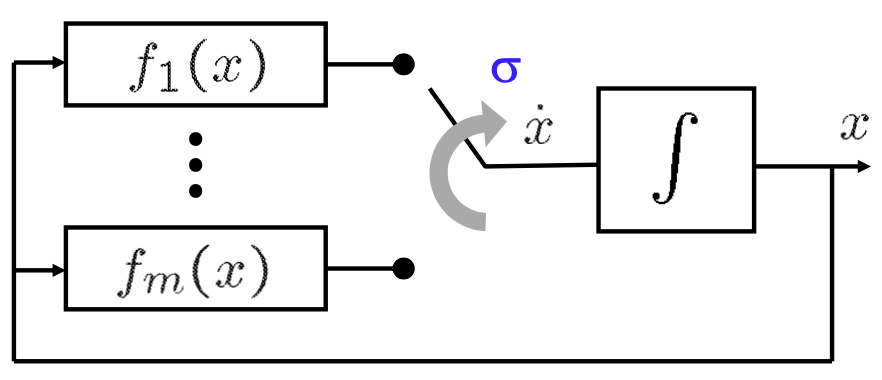
\includegraphics[width=0.7\linewidth]{immagini/swithced_1}
	\caption{Switched system}
	\label{fig:swithced1}
\end{figure}
A switched system can be compared to an hybrid system where the discrete transition mechanism (domains and guards) depends on the switching signal which can be state-dependent or time-dependent.
\begin{figure}[H]
	\centering
	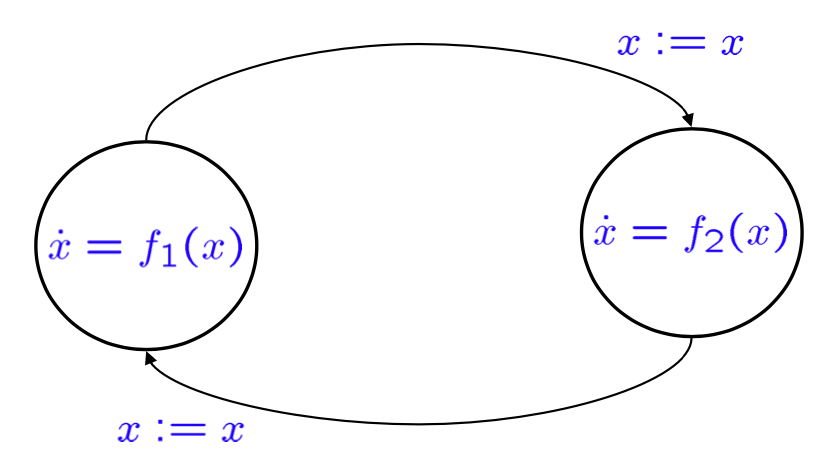
\includegraphics[width=0.7\linewidth]{immagini/swtich_hyb}
	\caption{$\dot{x}=f_{\sigma}(x), \sigma \in Q=\left\{1,2\right\}$}
	\label{fig:swtichhyb}
\end{figure}
\paragraph{State dependent switching example} The state space X is partitioned into operating regions, each one associated to the system is in action in that moment.  The system in action is specified by the switching system $\sigma(x)$.
\begin{figure}[H]
	\centering
	\includegraphics[scale=0.4]{immagini/state_d_sw}
	\caption{State-dependent}
	\label{fig:statedsw}
\end{figure}
\subparagraph{Example} Here is reported an example of a switched linear system.
\begin{figure}[H]
	\centering
	\includegraphics[scale=0.4]{immagini/s_l_S}
	\includegraphics[scale=0.4]{immagini/sls_2}
	\caption{Switching Linear System}
	\label{fig:sls2}
\end{figure}
The hybrid time set of the system in analysis is the following H=(Q,X,f,\textit{Init},Dom,E,G,R):
\begin{itemize}
	\item $Q=\left\{q_1,q_2\right\}$;
	\item $X=\Re^2$;
	\item $f(q_1,x)=A_1x$ and $f(q_2,x)=A_2x$; 
	\item $\emph{Init}=Q \times X$ 
	\item $Dom(q_1)=\left\{(x\in X\colon Cx>0\right\} $ and $Dom(q_2)=\left\{(x\in X\colon Cx\le0\right\} $;
	\item $E=\left\{(q_1,q_2),(q_2,q_1)\right\}$;
	\item$G((q_1,q_2))=\left\{(x\in X\colon Cx\le0\right\} $ and $G((q_2,q_1))=\left\{(x\in X\colon Cx>0\right\} $;
	\item$R((q_1,q_2),x)=R((q_2,q_1),x)=\left\{x \right\}$
\end{itemize}
\paragraph{Time dependent switching example} 
Meanwhile in time dependent switching system the \textcolor{red}{(exogenous) switching signal} is a piecewise constant function on time defined as $\sigma \colon \left[0,\infty\right) \to Q$. $\sigma(t)$ specifies the system that is active at time t.
\begin{figure}[H]
	\centering
	\includegraphics[scale=0.4]{immagini/s_td_s}
	\caption{$\dot{x}=f_{\sigma}(x), \sigma \colon \left[0,\infty\right) \to Q$} 
	\label{fig:stds}
\end{figure}
If the switching signal is abitrary (discrete transition method not specified), then H=(Q,X,f,\textit{Init},Dom,E,G,R):
 \begin{itemize}
	\item $Q=\left\{q_1,q_2\right\}$;
	\item $X=\Re^2$;
	\item $\emph{Init}=Q \times X$ 
	\item $f(q_1,x)=f_1(x)$ and $f(q_2,x)=f_2(x)$; 
	\item $Dom(q_1)=Dom(q_2)=X$;
	\item $E=\left\{(q_1,q_2),(q_2,q_1)\right\}$;
	\item$G((q_1,q_2))=G((q_2,q_1))=X$;
	\item$R((q_1,q_2),x)=R((q_2,q_1),x)=\left\{x \right\}$
\end{itemize}
In conclusion switched system with time-dependent arbitrary switching can be seen as a \textcolor{green}{higher-level abstraction of hybrid automata} where the discrete transition mechanism is not specified.
\subsection{Introduction to stability} \label{introstab}
We want now to start reasoning about the stability of a switched system and thus we need to define what is an equilibrium.
\begin{defn}[Equilibrium]
	Given a family of systems $\dot{x}=f_q(x), q\in Q=\left\{1,2,\dots,m\right\}$ with $f_q(0)=0, \forall q \in Q$: x=0 is an \textcolor{red}{equilibrium} of the switched system.
\end{defn}
Now it's important to study the stability of the equilibrium. Suppose to have a set of system with cardinality equal to two $\dot{x}=A_{\sigma}x$ where $\Re\left\{eigA_{\sigma}\right\}<0, \forall \sigma$ as shown in Figure \ref{fig:12stable} the two independent system are asymptotically stable.
\begin{figure}[H]
	\centering
	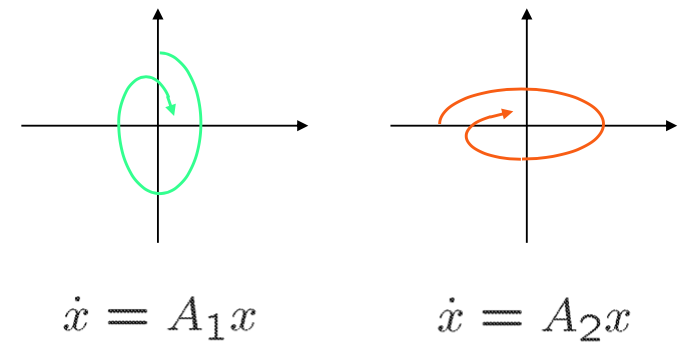
\includegraphics[scale=0.4]{immagini/1_2_stable}
	\caption{Stable trajectories}
	\label{fig:12stable}
\end{figure}
But depending on the switching signals we chose we can have different stability results, even instability of the overall switched system. Let's look what happens with the following example in Figure \ref{fig:12stable}
\begin{figure}[H]
	\centering
	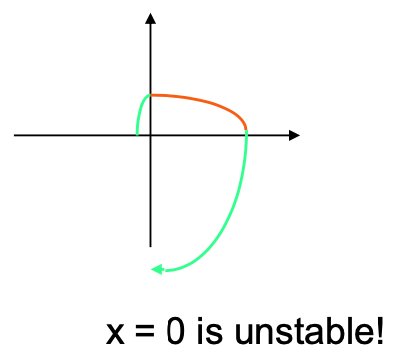
\includegraphics[scale=0.4]{immagini/sw_unstable}
	\includegraphics[scale=0.4]{immagini/sw_ast}
	\caption{Effect of the switching signal on stability}
	\label{fig:swunstable}
\end{figure}
Furthermore, some times even if we have a system of the set which is unstable the overall system can be asymptotically stable if the proper switching signal is chosen (or designed). An example follows in Figure \ref{fig:unst}
\begin{figure}[H]
	\centering
	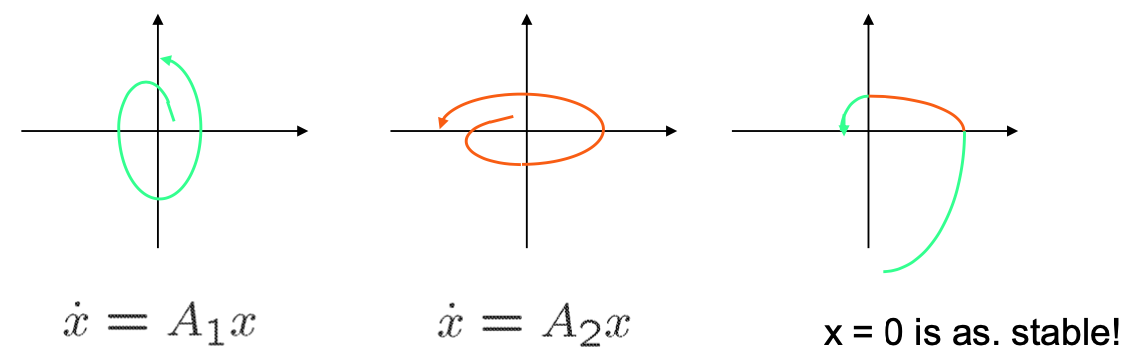
\includegraphics[scale=0.4]{immagini/un+st}
	\caption{Stabilizing with the switching signal}
	\label{fig:unst}
\end{figure}
\section{Stability for arbitrary switching}\label{stab-arb-sw}
In this section we will talk about how to reach global uniform asymptotic stability but before we have to give some definitions and theorems.

\begin{defn}[Globally uniformly asymptotically stable equilibrium]
	The equilibrium x=0 is \textcolor{green}{GUAS} if it is GAS, uniformly with respect to the switching signals $\sigma$.
\end{defn}
A \textcolor{green}{necessary condition for x=0 to be GUAS} is that $\dot{x}=f_q(x), q\in Q=\left\{1,2,\dots,m\right\}$ is a family of systems with GAS equilibrium in x=0.

\begin{defn}
	The family of systems $\dot{x}=f_q(x), q\in Q=\left\{1,2,\dots,m\right\}$ share a \textcolor{green}{common Lyapunov Function} at x=0 if there exists a continuously differentiable ($C^1$) function $V\colon\Re^n\to\Re$ such that \[
	 V(x)>0, \forall x \neq0, V(0)=0\quad \text{and} \quad \frac{\delta V}{\delta x}(x)f_q(x)<0, \forall x \neq0, \forall q \in Q
	 .\]
	 A common Lyapunov function at $x=0$ is quadratic if it is given by $V(x)=x^TPx$ with P symmetric and positive definite.
\end{defn}
\begin{thm}[Common Lyapunov function]\label{lyap-th}
	If the family of systems $\dot{x}=f_q(x), q\in Q=\left\{1,2,\dots,m\right\}$ share a \textcolor{red}{radially unbounded common Lyapunov function} $V\colon\Re^n\to\Re$ at x=0, then, the equilibrium x=0 is GUAS.
\end{thm}
\begin{thm}[Common \emph{quadratic} Lyapunov function] \label{quad-lyap-th}
	If there exists $P=P^T>0$ such that $PA_q+A_q^TP<0, \forall q \in Q= \left\{1,2,\dots,m\right\}$ then the equilibrium x=0 is GUAS.
\end{thm}
\begin{proof}
	$V(x)=x^TPx$ is radially unbounded common Lyapunov function at x=0.
\end{proof}
\begin{remark}
	The existence of a globally quadratic Lyapunov function is not necessary for x=0 to be GUAS.
\end{remark}

%%%5 there is an example but i need to listen the lesson%%%%
\subsection{Switched linear system with a special structure}
We now focus on a specific set of switched linear (the family of possible dynamics is linear) system which are characterized by matrices $A_q,\,q\in Q=\left\{1,2,\dots,m\right\}$ which are Hurwitz and:
\begin{itemize}
	\item commute
	\item are upper or lower triangular
\end{itemize}
\subsubsection{Commuting matrices}
So, considering, for example, for simplicity the case of $Q=\left\{1,2\right\}$ system defined by $\dot{x}=A_{\sigma}x$. Calling $s_k$ the time interval where $\sigma=1$ is activated and $t_k$ when $\sigma=2$ is activated the evolution of x(t) can be found thanks to Lagrange formula for each one dynamics.
\begin{figure}[H]
	\centering
	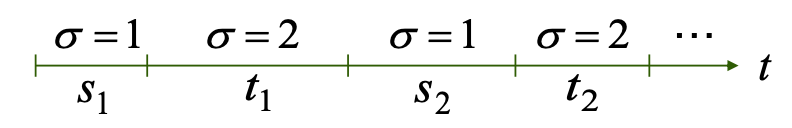
\includegraphics[scale=0.4]{immagini/bho}
	\caption{Arbitrary activation sequency}
	\label{fig:bho}
\end{figure}
\[
x(t)=e^{A_2t_k}e^{A_1s_k}\dots e^{A_2t_1}e^{A_1s_1}x(0)=e^{A_2(t_k+\dots +t_1)}e^{A_1(s_k+\dots +s_1)}x(0)\to 0
\] as $t\to\infty$.
We can also \textbf{prove the stability} building a common quadratic Lyapunov function. We firstly build a matrix $P_1$ which satisifies the Lyapunov equation and then plug in $P_1$ as the righten side of another Lyapunov equation in order to find $P_2$. So my statement is that $P_2$ build in such a way is the common quadratic Lyapunov function for the two linear system, one characterized by matrix $A_1$ and the other by matrix $A_2$.
\[
P_1A_1+A_1^TP_1=-I\]
\[
P_2A_2+A_2^TP_2=-P1
\]
So we can formalize as follow: $\exists\ a \ quadratic \ common \ Lyapunov \ function: V(x)=x^TP_2x$.First of all we know that if $A_1$ is Hurwitz there is an unique positive definite solution to the first Lyapunov equation which is $P_1$ and when we plug in $P_1$ in the second equation the same consideration apllies because also $A_2$ is Hurwitz. Where $P_1$ and $P_2$ are as follows:
\[P_2=\int_{0}^{\infty} e^{A_2^Tt}P_1e^{A_2^Tt}\, dt \qquad P_1=\int_{0}^{\infty} e^{A_1^Tt}Ie^{A_1^Tt}\, dt\]
Now plugging in the first expression in the second, and commuting the exponential (to be clear, switching $A_1$ and $A_2$) one we obtain: 
\[P_2=\int_{0}^{\infty} e^{A_1^T\tau}\underbrace{\int_{0}^{\infty} e^{A_2^Tt}Ie^{A_2^Tt}\, dt}_{Q}e^{A_1^T\tau}\, d\tau
\]
And so we can notice that $P_2$ satisfies also the following Lyapunov equation for the dynamic $A_1$:
\[
P_2A_1+A_1^TP_2=-Q.
\]
\subsubsection{Triangular Hurwitz matrices}
	\[
	\dot{x}_1=\lambda_{1,\sigma}x_1+a_{\sigma}x_2\]
	\[
	\dot{x}_!=\lambda_{2,\sigma}x_2
	\]
We know that the two $\lambda$ since the matrices are Hurwitz should be strictly negative. We notice that the second equation is independent from the first one so we can compute the evolution of $x_2(t)$ as we did in the previous chapter. So we know that $x_2(t)$ is the product of many exponential but the exponentials of a scalar which are indeed the eigenvalues $\lambda$. Thus when I found an upper bound I can say that the absolute value of $x_2(t)$ is less or equal to the exponential with the lowest rate of decrease which is the one associated to the large eigenvalue among every dynamics eigenvalues. In conclusion $x_2(t)$ goes to zero because all eigenvalue are strictly negative.
\[
\dot{x}_2=\lambda_{2,\sigma}x_2 \Rightarrow \left|x_2(t)\right|\le e^{\max_p\lambda_{2,p}t}\left |x_2(0)\right| \to 0
\]
\[
\boxed{\dot{x}_1=\lambda_{1,\sigma}x_1}+\boxed{a_{\sigma}x_2}\Rightarrow x_1(t)\to 0
\]
The same thing can be said for the first equation. Here $x_2(t)$ can see as an input that goes to zero. The first part is an \underline{exponentially stable system} while the second part is, as we demonstrated previously, a \underline{exponentially decaying perturbation} so tends to zero as t tends to infinity.

\section{Stability for constrained switching}
The main difference between arbitrary and constrained switching is that now we can select the way we switch from one dynamic to the other  in such a way we get global asymptotical stability for the zero equilibrium. Notice that we can't get anymore uniform stability.
\subsection{Stability under slow switching}
Supposing to have a linear system, (can be extended to nonlinear) the matrices we are given are Hurwitz but as we saw in \ref{introstab} even if the matrices are Hurwitz we are not guarantied of the preserving of stability. So the idea here goes as follow: if each dynamic is asymptotically stable, if you stay long enough with one dynamic activated you are going to have a contraction of the value of the state x(t) because, eventually, as the time goes to infinity the state will tend to zero. So at this point if we initialize the absolute value of $\left\|x(0)\right\|$ at a certain value if we wait enough, before switching to the other dynamic, (because there can be overshoots) the absolute value $\left\|x(t)\right\|$ will become smaller then $\left\|x(0)\right\|$). This waiting time is called \textbf{dwell time} $\tau_D$. So the choice of $\tau_D$ is crucial for the preservation of global asymptotic stability. Let's prove it more formally.
Starting from the computation of $x_(t)$ as we did before:
\[x(t)=e^{A_2t_k}e^{A_1s_k}\dots e^{A_2t_1}e^{A_1s_1}x(0)\]
and applying the absolute value to both sides, the relation still holds:
\[\|x(t)\|=\|e^{A_2t_k}e^{A_1s_k}\dots e^{A_2t_1}e^{A_1s_1}x(0)\|.\]
Now the idea is to upper bound this expression with the product of the norm of the exponentials of the matrices:
\[\|x(t)\| \le \| e^{A_2t_k}\| \|e^{A_1s_k}\dots e^{A_2t_1}e^{A_1s_1}x(0)\|.\]
This is possible thanks to the definition of the norm which I'm recalling here:
\begin{defn}[Norm] \label{norm}
	\[\|M\| = \sup_{y \neq0}\frac{\|My\|}{\|y\|}\to \|My\| \le \|M\|\|y\|
	\]
\end{defn}
And iterating the procedure we finish into:
\[\|x(t)\| \le \| e^{A_2t_k}\| \|e^{A_1s_k}\|\dots \|e^{A_2t_1}\|\|e^{A_1s_1}\|\|x(0)\|.\]
So, again applying the Definition \ref{norm}, we have:
\begin{equation}\label{eq1}
	\|e^{At}\|=\sup_{x_0 \neq0}\frac{\|e^{At}x_0\|}{\|x_0\|}\le \mu e^{-\lambda_0t},t \ge 0
\end{equation}
Where this $\lambda_0$ is a positive number that has to be smaller then the minimum absolute value of the real part of all eigenvalues. This is the \emph{lowest decay rate} so that the inequality holds for all dynamics.
How can I chose given all this information $\tau_D$? 
\begin{equation} \label{eq2}
	\tau_D \ge \frac{\log\mu}{\lambda_0-\lambda} \text{ with } \lambda\in(0,\lambda_0)\Longrightarrow \mu \le e^{\tau_D(\lambda_0-\lambda)}
\end{equation}

So now plugging the expression of $\mu$ found in \ref{eq2} in \ref{eq1} we obtain:
\begin{equation} \label{eq3}
	\|e^{A_i\Delta t}\| \le \mu e^{-\lambda_0\Delta t}\le e^{\tau_D(\lambda_0-\lambda)}e^{-\lambda_0\Delta t}
\end{equation}
and since $\Delta t \ge \tau_D$ and $\lambda_0 > \lambda$ we can upperbound and simplify as follow:
\begin{equation}
 		\|e^{A_i\Delta t}\| \le \mu e^{-\lambda_0\Delta t}\le e^{\tau_D(\lambda_0-\lambda)}e^{-\lambda_0\Delta t} \le e^{\Delta t(\lambda_0-\lambda)}e^{-\lambda_0\Delta t}=\boxed{e^{-\lambda t}\|x(0)\|}
\end{equation}
Here $\lambda_0$ is the \textbf{exponential rate of convergence} and should not be higher then maximum eig(A-LC). So we not only have global asymptotic stability but also \textbf{global exponential stability}.
\begin{remark}
	$\tau_D$ can be tailored to each time interval associated to each single dynamic independently.
\end{remark}
\section{Stability under state-dependent switching}
If since now we have studied the stability property of a time-dependent switching system, in this section we will show some result on how to prove or enforce stability of a state-dependent switching system.
\linebreak[2]
\begin{figure}[H]
	\centering
	\includegraphics[scale=0.4]{immagini/ss-ds}
	\caption{State-dependent switching system in the partitioned state space}
	\label{fig:ss-ds}
\end{figure}
Suppose we have given a switching rule and the partition of state space as in section \ref{fig:ss-ds}. In every part of the state space we have an associated dynamic. How can we prove the stability of the zero equilibrium? We start exploiting the following notion of state-dependent common Lyapunov function.
\begin{defn}[state-dependent common Lyapunov function]
	The family of systems $\dot{x}=f_q(x), x \in \Re^n, q \in Q=\left\{1,1,\dots,m\right\}$ has a \textcolor{green}{state-dependent common Lyapunov function} at x=0 if there exists a $C^1$ function $V\colon \Re^n\to\Re$ such that
	\[
	V(x)>0, \forall x\neq 0, V(0)=0	
		, \forall x \in \Re^n
	\]
	where $\sigma\colon X \to Q$.
\end{defn}

 We can notice that this is a less strict requirement then the one of common quadratic Lyapunov function stated in Theorem \ref{quad-lyap-th}. Why? Here the dynamic should decrease only in the state space region in which is activated. For example in figure \ref{fig:ss-ds} the function $f_1(x)$ is not required to be decreasing when we are in $X_3$.\\
 A theorem can be derived:
\begin{thm}
	Given the system $\dot{x}=f_{\sigma}(x), \sigma\colon X\to Q$, if there exists a radially unbounded state-dependent common Lyapunov equation at x=0 for the switched system, then, the equilibrium x=0 is GAS.
\end{thm}
\begin{remark}
	need that $\frac{\delta V}{\delta x}(x)f_{\sigma(x)}(x)<0$ only when $\sigma$ is equal to q. So in the switched linear case matrices $A_q$ are not required to be Hurwitz.
\end{remark}
\subsection{Stabilization by switching}
It is possible given two (or more) unstable linear system to build a state dependent switching rule that makes the zero equilibrium GAS. The trick is basically to build a state-dependent switching rule such that there exists a common Lyapunov function for this two dynamics of the system.\\ This is possible if:
\begin{thm}
	If the matrices $A_1$ and $A_2$ have a convex Hurwitz combination, then, there exists a state-dependent switching strategy such that the equilibrium x=0 of the switching system $\dot{x}=A_{\sigma(x)}x$ is GAS.
\end{thm}

But what does it mean \emph{convex combination}? Let's do an example:
\paragraph{Example} Considering $\dot{x}=A_1x$ and $\dot{x}=A_2x$ both unstable, assume:
\[
A=\alpha A_1+(1-\alpha)A_2 \text{ Hurwitz for some } \alpha \in (0,1)
\]
This is a \emph{convex} combination because the selected parameters are between zero and one and sum up to one. Since A is Hurwitz there exists a matrix P such that Lyapunov inequality is satisfied
\[
A^TP+PA<0.
\]
Now we put in place of A the first expression defined as an assumption:
\[
\alpha(A_1^TP+PA_1)+(1-\alpha)(A_2^TP+PA_2)<0
\]so for each $x\neq0$ either
\[
\underbrace{x^T(A_1^TP+PA_1)x<0}_{\text{define region $X_1$ where system 1 is active}} \ \textbf{or} \ \underbrace{x^T(A_2^TP+PA_2)x<0}_{\text{define region $X_2$ where system 2 is active}}
\]
We notice that the above inequality come from the derivative of the Lyapunov function $V(x)=x^TPx$ along the two dynamics. So we activate the dynamic when V decreases. So practically we enforce V(x) to be a common quadratic Lyapunov function.
$V(x)=x^TPx$ is a radially unbounded state-dependent common Lyapunov function at x=0 for $\dot{x}=A_{\sigma(x)}x$ $\Longrightarrow$ x=0 is GAS.
In conclusion: what is the shape of this two regions? There are conic regions because for example taking a random point in yellow region, every point on the line that pass trough the point and the origin satisfies the same inequality because they can be parametrized  as a function of $\bar{x}$ as $K\bar{x}$ and if we put $K\bar{x}$ in the fuction above we get $K^2$ that multiplies the other part of the expression and doesn't change the sign of it.
\begin{figure}[H]
	\centering
	\includegraphics[scale=0.4]{"immagini/conic regions"}
	\caption{$X_1$ is the yellow region, $X_2$ is the green one.}
	\label{fig:conic-regions}
\end{figure}
Notice that the two parts partially overlap because they can't be just complementary because the boundary cannot belong to any region (strict inequality) so they should overlap at least a bit.
\section{Observer design}
The goal of an observer is to recover the state of a system from its input and output.\begin{figure}[H]
	\centering
	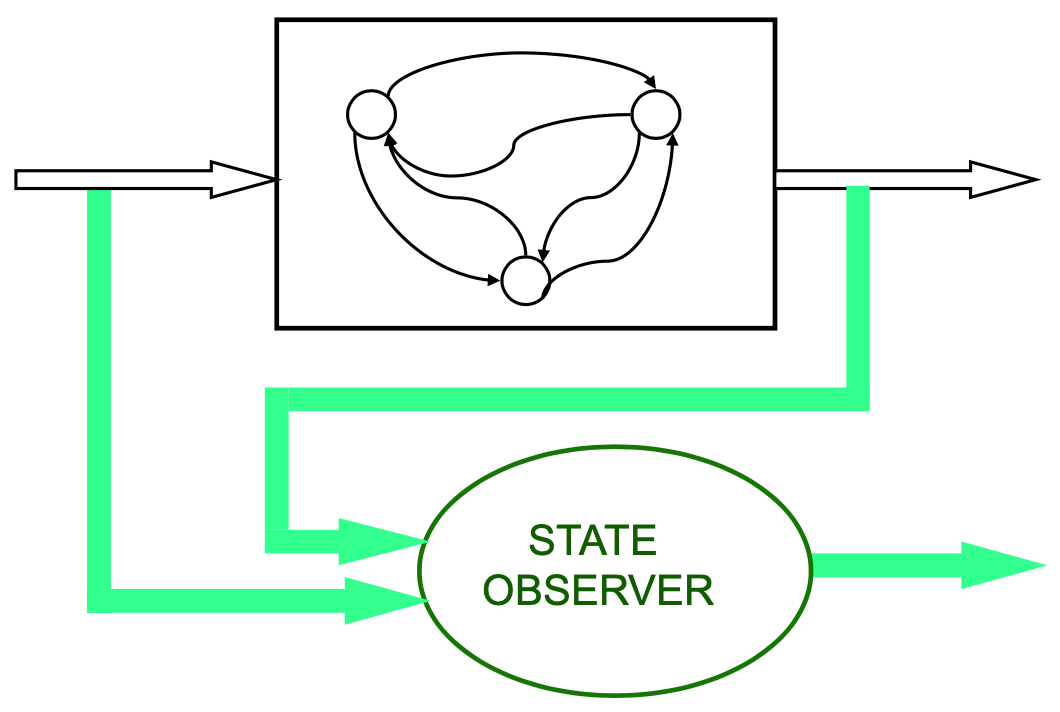
\includegraphics[scale=0.35]{immagini/obs}
	\caption{State observer}
	\label{fig:obs}
\end{figure}
We will firstly have a look to the problem of observer design for \emph{continuous time linear systems} and then transpose the concepts to \emph{switched linear systems} with switching signal available through measurements.
\subsection{Observer design for continuous time linear system}
The system we are dealing with is of the form:
$\begin{cases} 
	\dot{x}(t)=Ax(t)+Bu(t)\\
	y(t)=Cx(t)\\
\end{cases}$
where 
\begin{itemize}
	\item[] $u(t)\in \Re^m \equiv input$
	\item[] $y(t)\in \Re^p \equiv output$
	\item[] $x(t)\in \Re^n \equiv state$.
\end{itemize}
	\begin{figure}[H]
	\centering
	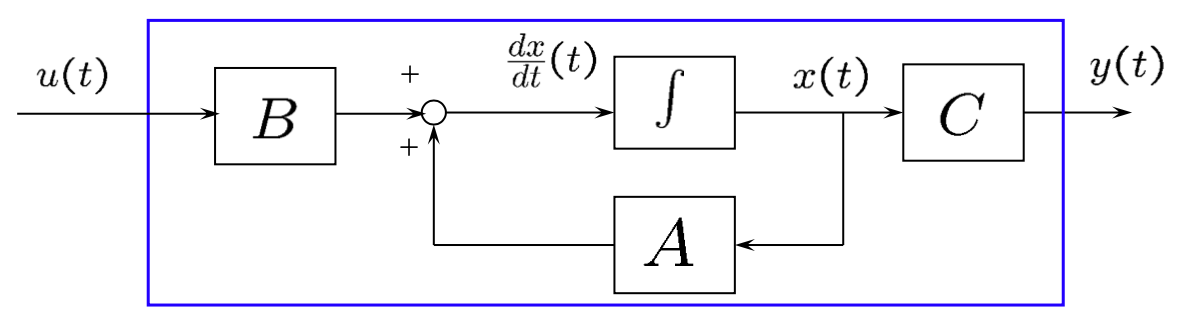
\includegraphics[scale=0.4]{immagini/cont-lin-sys}
	\caption{Continuous linear system}
	\label{fig:cont-lin-sys}
\end{figure}
\begin{defn}[Asymptotic or Lurenberger observer]
	An asymptotic observer is a system that consistently estimates the state x(t) based on the input and output measurements $u(\tau)$ and $y(\tau), 0 \le \tau \le t$, for any (unknown) initial condition $x_0$ and for any input $u(\cdot):$
	\[
	\lim_{t\rightarrow \infty}\|\hat{x}(t)-x(t)\|=0, \qquad \forall x(0)=x_0\in \Re^n, \forall u(\cdot)
	\]
\end{defn}
Essentially the observer is a copy of the original system with an extra exogenous input which depends on the output of the real system.
\begin{figure}[H]
	\centering
	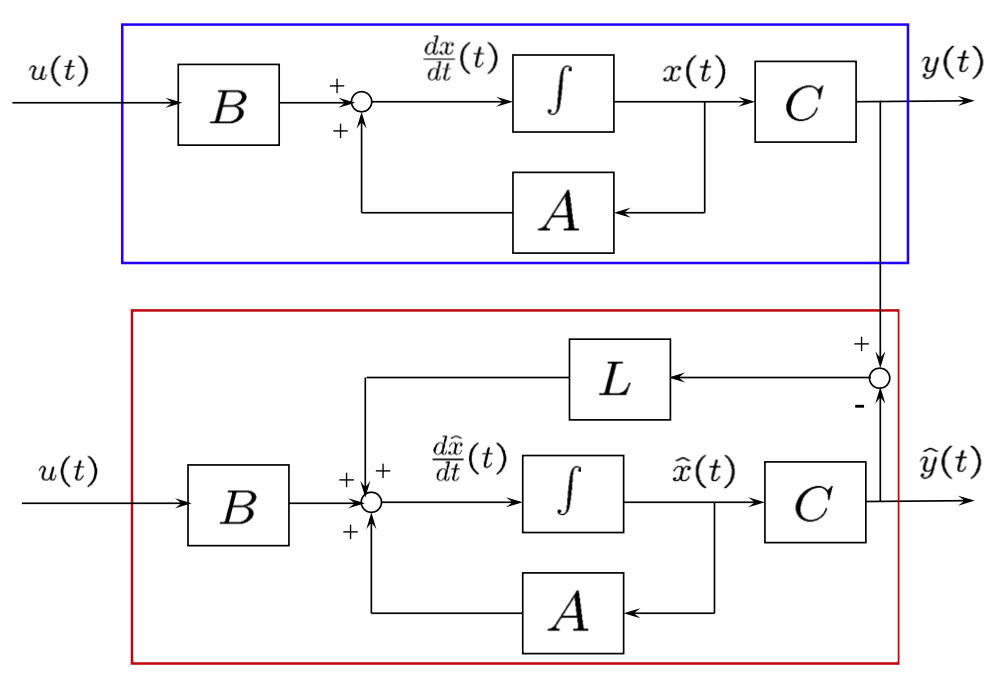
\includegraphics[scale=0.4]{immagini/observer}
	\caption[Asymptotic observer]{}
	\label{fig:observer}
\end{figure}
The equation of the observer is then:
\[
\begin{cases} 
	\dot{\hat{x}}(t)=A\hat{x}(t)+Bu(t)+\textcolor{red}{L}(y(t)-\hat{y}(t))\\
	\hat{y}(t)=C\hat{x}(t)\\
\end{cases}
\]
Defining the prediction state error $e(t)\colon= x(t)-\hat{x}(t)$ we complete the observer system result:
\[
\begin{cases} 
	\dot{\hat{x}}(t)=A\hat{x}(t)+Bu(t)+\textcolor{red}{L}(y(t)-\hat{y}(t))\\
	\hat{y}(t)=C\hat{x}(t)\\
	\dot{e}(t)=(A-LC)e(t)\\
\end{cases}
\]
If A is Hurwitz, then,
\begin{itemize}
	\item one can set L=0 and obtain that the estimation error converges exponentially to zero because when my system is asymptotically stable the contribution of the initial condition (which is unknown) goes to 0 so basically we don't need to reconstruct $x_0$;
	\item no output measurements are needed, but the rate of convergence will be determined by the real part of the eigenvalues of A.
\end{itemize}
But what if A is not asymptotically stable?
\begin{thm}
	If the couple (A,C) is detectable, then, L can be designed so that A-LC is Hurwitz and, hence, the estimation error converge exponentially to zero:
	\[
	\|e(t)\| \le \mu e^{-\lambda_0t}\|e(0)\|, t\ge 0, \qquad \forall e(0)=e_0 \in \Re^n
	\]
\end{thm}
In order to define the concept of detectability we need to define first the \textbf{observability} property:
\begin{defn}[Observable system]
	A system is observable if all states $x\neq0$ are observable that means that the observability matrix $O_n$ has maximum rank (n).
	\[
	O_n=\begin{bmatrix} 
		C \\
		CA\\
		CA^2\\
		\vdots\\ 
		CA^{n-1}
    \end{bmatrix}
	\]
\end{defn}
The key property is that if the couple (A,C) is observable one can select matrix L such that A-LC has arbitrarily chosen eigenvalues.

\begin{defn}
	A system is detectable if the eigenvalues of the unobservable parte have all striclty negative real part.\\
	In this case, the pair \textcolor{red}{(A,C)} is \textcolor{red}{detectable}.
\end{defn}
\subsubsection{Sketch of the proof}
Assume without loss of generality that the system is in the observable canonical form. If not, then we can use Kalman decomposition:  $w\colon=T_ox$
\begin{figure}[H]
	\centering
	\includegraphics[scale=0.4]{immagini/proof}
	\label{fig:proof}
\end{figure}
\[\begin{bmatrix}
	\dot{w}_o(t)\\
	\dot{w}_{no}(t)
\end{bmatrix}
=\begin{bmatrix}
	A_{11} & 0\\A_{21} & A_{22}
\end{bmatrix}\begin{bmatrix}
w_o(t)\\w_{no}(t)
\end{bmatrix}
+\begin{bmatrix}
	B_1\\B_2
\end{bmatrix}u(t)
\]
\[
y(t)=\begin{bmatrix}
	C_1 & 0
\end{bmatrix}\begin{bmatrix}
w_0(t)\\w_{no}(t)
\end{bmatrix}
\]
The dynamics of the estimation error is:
\[
\dot{e}(t)=\left(A-LC\right)e(t)\\
e_w\colon=T_oe
\]
and so
\[
\dot{e}_w(t)=\left( \begin{bmatrix}
	A_{11} & 0\\A_{21} & A_{22}
\end{bmatrix}-\begin{bmatrix}
	\tilde{L}_1 \\ \tilde{L}_2
\end{bmatrix} \begin{bmatrix}
C_1 & 0
\end{bmatrix}\right) e_w(t)=\begin{bmatrix}
	\boxed{A_{11}-\tilde{L}_1C_1} & 0\\
	A_{21}-\tilde{L}_2C_1 & \boxed{A_{22}}
\end{bmatrix} e_w(t)
\]
where $\tilde{L}=T_oL$.\\
The eigenvalues of $A_{11}-\tilde{L}_1C_1$ can be arbitrarily selected since $\left( A_{11},C_1\right)$ is observable and the eigenvalues of the unobservable part ($A_{22}$) are being keep fixed.
\begin{thm}
	If (A,C) is detectable, then, L can be designed so that A-LC is Hurwitz and, hence, the estimaton error converges exponentially to zero:
	\[
		\|e(t)\| \le \mu e^{-\lambda_0t}\|e(0)\|, t\ge 0, \qquad \forall e(0)=e_0 \in \Re^n
	\]
\end{thm}
\begin{remark}
	The convergence rate can be arbitrarily chosen if and only if (A,C) is observable.
\end{remark}
\subsection{Observer design for switched linear system}
Since we have a switching signal that at every time t dictate which system is active we have a kind of discrete system and two outputs.
\newline
Having the following kind of system:
\[
\dot{x}(t)=A_{\sigma(t)}x(t)+B_{\sigma(t)}u(t)\]
\[
y(t)=C_{\sigma(t)}x(t)
\]
and the switching occurs within the family of systems:
\[
\dot{x}(t)=A_qx(t)+B_qu(t) \]
\[
y(t)=C_qx(t)
\] with $ q=\left\{1,2,\dots,m\right\}$\\
\textcolor{red}{Assumptions:}
\begin{enumerate}
\item[(i)] the switching signal $\sigma\colon \left[0,\infty\right)\to Q$ is available as (discrete) output signal
\item[(ii)] $(A_q,C_q)$ is detectable for all $q\in Q$
\end{enumerate}
The idea here is the same as for linear system but we need to design an observer for each system that activate when the system is activated by the switching system.
\begin{figure}[H]
	\centering
	\includegraphics[scale=0.55]{immagini/s_ob}
	\caption{Switching observer}
	\label{s_on}
\end{figure}
As did before now we derive the dynamics of the estimation error from the system and observer equations:
\[\text{system}\colon \begin{cases}
	\dot{x}(t)=A_{\sigma(t)}x(t)+B_{\sigma(t)}u(t)\\
	y(t)=C_{\sigma(t)}x(t)
\end{cases}
\]
\[\text{observer}\colon \begin{cases}
	\dot{\hat{x}}(t)=A_{\sigma(t)}\hat{x}(t)+B_{\sigma(t)}u(t)+L_{\sigma(t)}(y)(t)-\hat{t}(t))\\
	y(t)=C_{\sigma(t)}x(t)
\end{cases}
\]
\[
\boxed{\dot{e}(t)=\left( A_{\sigma(t)}-L_{\sigma(t))}C_{\sigma(t)}\right)e(t)}
\]
\begin{thm}
	If there exists $P=P^T>0$ such that \[P(A_q-L_qC_q)+(A_q-L_qC_q)^TP<0, \forall q \in Q=\left\{1,2,\dots,m\right\}\] then, the switching observer consistently estimates the continuous state of the switched system, for any e(0) and for any $\sigma \colon \left[0,\infty\right) \to Q$.
\end{thm}

\begin{proof}
	 $V(e)=e^TPe$ is a radially unbounded common Lyapunov function at the equilibrium e=0. Then, e=0 is GUAS.
	\end{proof}
\paragraph{Switching observer design}
At this point we have to concretely design the observer and so its gains. The gains $L_1,L_2,\dots,L_m$ such that there exist $P=P^T>0$ satisfying: \[P(A_q-L_qC_q)+(A_q-L_qC_q)^TP<0, \forall q \in Q=\left\{1,2,\dots,m\right\}
\]
Since the product between P and $L_q$ makes the system non linear so we have to do a \textcolor{red}{Linear Matrix Inequalities (LMI) reformulation}.
By setting $L_q=P^{-1}Y_q$, we have $PL_q=Y_q$ the problem can then be rephrased as that of determining $P=P^T>0$ and $Y_1,Y_2,\dots,Y_m$ such that \[
PA_q-Y_qC_q+A_q^TP-C_q^TY_q^T<0, \forall q \in  Q =\left\{1,2,\dots,m\right\}
\]
Gains are then recovered by $L_q=P^{-1}Y_q$.
The implementation idea is to design the switching observer gains $L_1,L_2,\dots,L_m$ such that the dynamics of the estimation error $\dot{e}(t)=(A_{\sigma(t)}-L_{\sigma(t)}C_{\sigma(t)})e(t)$ is contractive over each switching time interval, and, hence $e(t)\to 0$, for any e(0) and for any $\sigma \colon \left[0,\infty\right)\to Q$ with minimum dwell time $\tau_D$.
\begin{remark}
	Stability under slow switching condition is forced by making the error dynamics fast compared with the given $\tau_D$.
\end{remark}
To do this in practice we have to relay on the \textbf{squashing lemma}:\\
Suppose (A,C) observable. Let $\tau_D>0$. Then, for any $\rho >0$ there exist $\alpha>0$ and L such that \[\|e^{(A-LC)t}\| \le \rho e^{-\alpha(t-\tau_D)}, t \ge 0\]
If one chooses $0<\rho<1$, then, the dynamics is contractive over each time interval of length larger than or equal to $\tau_D$. So it's crucial to know the length of the dwell time in order to design L. The system converges exponentially and if after a certain time the system doesn't switch anymore it is still stable and converging because is Hurwitz.
%%% Fine del capitolo%%%